\documentclass[aps,twocolumn,secnumarabic,balancelastpage,amsmath,amssymb,nofootinbib]{revtex4}
% \documentclass[aps,twocolumn,secnumarabic,balancelastpage,amsmath,amssymb,nofootinbib]{revtex4}

% Documentclass Options

% nobalancelastpage doesn't attempt to equalize the lengths of the two columns
% on the last page as might be desired in a journal where articles follow one
% another closely
% amsmath and amssymb are necessary for the subequations environment among
% others secnumarabic identifies sections by number to aid electronic review
% and commentary. nofootinbib forces footnotes to occur on the page where they
% are first referenced and not in the bibliography

% \usepackage{lgrind}        % convert program listings to a form includable in a LaTeX document
\usepackage{chapterbib}    % allows a bibliography for each chapter (each labguide has it's own)
\usepackage{color}         % produces boxes or entire pages with colored backgrounds
\usepackage{graphics}      % standard graphics specifications
\usepackage[pdftex]{graphicx}      % alternative graphics specifications
\usepackage{longtable}     % helps with long table options
\usepackage{epsf}          % old package handles encapsulated post script issues
\usepackage{bm}            % special 'bold-math' package
\usepackage{tikz}
\usepackage{asymptote}     % For typesetting of mathematical illustrations
\usepackage{subfigure}

% \usepackage{thumbpdf}

\usepackage[colorlinks=true]{hyperref}  % this package should be added after all others
% use as follows: \url{http://web.mit.edu/8.13}
\newcommand{\drelectron}[1]{\node at #1 [circle, draw, inner sep=0pt, minimum size=1pt] {\_}}
\newcommand{\ud}{\mathrm{d}}
\newcommand{\ue}{\mathrm{e}}
\newcommand{\ui}{\mathrm{i}}
\newcommand{\res}{\mathrm{Res}}
\newcommand{\Tr}{\mathrm{Tr}}
\newcommand{\dsum}{\displaystyle\sum}
\newcommand{\dprod}{\displaystyle\prod}
\newcommand{\dlim}{\displaystyle\lim}
\newcommand{\dint}{\displaystyle\int}
\newcommand{\fsno}[1]{{\!\not\!{#1}}}
\newcommand{\eqar}[1]
{
  \begin{align*}
    #1
  \end{align*}
}
\newcommand{\texp}[2]{\ensuremath{{#1}\times10^{#2}}}
\newcommand{\dexp}[2]{\ensuremath{{#1}\cdot10^{#2}}}
\newcommand{\eval}[2]{{\left.{#1}\right|_{#2}}}
\newcommand{\paren}[1]{{\left({#1}\right)}}
\newcommand{\lparen}[1]{{\left({#1}\right.}}
\newcommand{\rparen}[1]{{\left.{#1}\right)}}
\newcommand{\abs}[1]{{\left|{#1}\right|}}
\newcommand{\sqr}[1]{{\left[{#1}\right]}}
\newcommand{\crly}[1]{{\left\{{#1}\right\}}}
\newcommand{\angl}[1]{{\left\langle{#1}\right\rangle}}
\newcommand{\tpdiff}[4][{}]{{\paren{\frac{\partial^{#1} {#2}}{\partial {#3}{}^{#1}}}_{#4}}}
\newcommand{\tpsdiff}[4][{}]{{\paren{\frac{\partial^{#1}}{\partial {#3}{}^{#1}}{#2}}_{#4}}}
\newcommand{\pdiff}[3][{}]{{\frac{\partial^{#1} {#2}}{\partial {#3}{}^{#1}}}}
\newcommand{\diff}[3][{}]{{\frac{\ud^{#1} {#2}}{\ud {#3}{}^{#1}}}}
\newcommand{\psdiff}[3][{}]{{\frac{\partial^{#1}}{\partial {#3}{}^{#1}} {#2}}}
\newcommand{\sdiff}[3][{}]{{\frac{\ud^{#1}}{\ud {#3}{}^{#1}} {#2}}}
\newcommand{\tpddiff}[4][{}]{{\left(\dfrac{\partial^{#1} {#2}}{\partial {#3}{}^{#1}}\right)_{#4}}}
\newcommand{\tpsddiff}[4][{}]{{\paren{\dfrac{\partial^{#1}}{\partial {#3}{}^{#1}}{#2}}_{#4}}}
\newcommand{\pddiff}[3][{}]{{\dfrac{\partial^{#1} {#2}}{\partial {#3}{}^{#1}}}}
\newcommand{\ddiff}[3][{}]{{\dfrac{\ud^{#1} {#2}}{\ud {#3}{}^{#1}}}}
\newcommand{\psddiff}[3][{}]{{\frac{\partial^{#1}}{\partial{}^{#1} {#3}} {#2}}}
\newcommand{\sddiff}[3][{}]{{\frac{\ud^{#1}}{\ud {#3}{}^{#1}} {#2}}}

\begin{document}
\tikzstyle{every picture}+=[remember picture]
\title{Measurement of hyperfine structure using Doppler-free saturated absorption spectroscopy.}
\author{Yichao Yu}
\email{yuyichao@mit.edu}
\homepage{http://yyc-arch.org/}
\date{\today}
\affiliation{MIT Department of Physics}

\begin{abstract}
  The Doppler-free saturated absorption spectroscopy is a technique to measure optical frequency absorption spectrum without affected by Doppler broadening based on the saturated absorption effect. Because of the higher resolution provided by this technique, it can be used to measure the fine and hyperfine structure of atomic energy levels as well as stabilize laser frequency using certain atomic lines. In this experiment, the Doppler-free spectrum was measured for the $D_2$ lines of ${}^{85}Rb$ and ${}^{87}Rb$ and the hyperfine structure constants of these lines are calculated.
\end{abstract}

\maketitle
%%%%%%%%%%%%%%%%%%%%%%%%%%%%%%%%%%%%%%%%%%%%%%%%%%%%%%%%%%%%%%%%%%
\section*{Introduction}
When measuring the spectrum of certain material, there are different effects that can broaden the line width and affect the precision of the measurement. For the optical frequency spectrum measurement at room temperature, the first broadening effect is the natural linewidth causing by the finite lifetime of the state due to the interaction with vacuum fluctuation. Since there is not possible now to change vacuum fluctuation and increase the lifetime of the excited state, this broadening effect cannot be eliminate. Another usually larger but less interesting effect is the Doppler broadening causing by the motion of atoms at non-zero temperature given by,
\[ \Delta f\approx\sqrt{\frac{k_BT}{mc^2}}f_0 \]
For the Rubidium $D_2$ lines we are measuring in this experiment, the Doppler broadening is about $200MHz$, about $30$ times larger than the natural linewidth ($\approx6MHz$). One way to eliminate the Doppler broadening is to cool down the temperature of the sample. However, either cool down the whole sample or using a collimated beam to achieve a low transverse temperature need some more or less complicated experiment setup. Another way to do a Doppler-free measurement of the spectrum, which is the saturated absorption spectroscopy, was predicted and discovered by Bennett in the early 1960s when he was studying the fluorescence of a narrow line-width $He-Ne$ laser \cite{he_ne_hole}. This method has a relatively simpler setup and can also works in room temperature.

In this experiment, we measured the saturated absorption spectrum of ${}^{87}Rb$ and ${}^{85}Rb$ $D_2$ lines. Hyperfine splitting in both the excited state and ground state are observed and the hyperfine splitting constants are calculated and compared to the expected value.

\section{Theory.}
\subsection{Saturated absorption.}
When shining atoms with resonant light, the light will be absorbed and scattered by the atoms. At the same time, the atoms will undergo a Rabi flopping between the excited and ground states as well as spontaneous decay from the excited state. For low light intensity from a non-laser normal light source, the spontaneous decay is the dominant effect and the most of the atoms will stay in their ground state. However, for a laser beam with a high intensity, the coherent transition driven by the laser will be comparable or larger than the spontaneous emission. As a result, the Rabi flopping will dominant and on average half of the atoms will be pumped by the laser beam to the excited state. The intensity for this to happen is called saturation intensity. Above this intensity, the atoms have already reached their maximum capability of scattering light, i.e. spontaneous emission or absorption, therefore if we continue increasing the intensity of the beam, the scattering or absorption power will not increase anymore, i.e. the absorption is saturated.

\subsection{Saturated absorption spectroscopy.}
Saturated absorption spectroscopy is a technique to measure the Doppler free spectrum using velocity selection based on saturated absorption.
\subsubsection{Lamb dip and velocity selection.}
For a single laser beam, the saturated absorption effect only imposes a maximum absorption for the beam. However, if a second laser beam is added, since the transition is already saturated by one beam, if the two beams are in resonance with the same group of atoms, a decrease, which is called Lamb dip, in the absorption of both beams can be observed because of the saturation.

In the setup of saturated absorption spectroscopy, two beams are counterpropagating and are of the same frequency $\nu_0$. The frequencies of the two beams for atoms with a Doppler shift $\Delta_{Doppler}$ in the beam axis are,
\eqar{
  \nu_{1,2}=&\nu_0\pm\Delta_{Doppler}
}
For the lamb dip to appear for a transition of frequency $\nu$, the atoms needs to be in resonance with both beams, i.e.,
\eqar{
  &\nu_1=\nu_2=\nu\\
  &\Delta_{Doppler}=0\\
  &\nu_0=\nu
}
Since only atoms with $\Delta_{Doppler}=0$, i.e. zero velocity along the beams, are selected and contribute to the effect, the Lamb dip is not affect by Doppler broadening.
\subsubsection{Multiple excited states and crossover dips.}
When there are multiple excited states in the atom, there can be crossover dips in the middle of each two excited states. If the atoms are in resonance with the two beams on the transitions to two different excited states, a crossover dips will appear since the atoms are pumped away by one beam decreasing the absorption of the other beam. The condition for this crossover peak with the saturated spectroscopy setup on two transitions with frequencies $\nu$ and $\nu'$ is,
\eqar{
  \nu=&\nu_0\pm\Delta_{Doppler}\\
  \nu'=&\nu_0\mp\Delta_{Doppler}
}
Therefore,
\eqar{
  &\Delta_{Doppler}=\pm\frac{\nu-\nu'}{2}\\
  &\nu_0=\frac{\nu+\nu'}{2}
}

Since these crossover dips involves two groups of atoms (two possible $\Delta_{Doppler}$), they are generally larger than the depth of the Lamb dips corresponding to any of the two original states, which make them helpful for the experiment. When measuring the spectrum using saturated absorption, the height of different dips may not be the same due to different dipole moments and different degrees of degeneracy and some dips may not be easily visible. In such cases, we can use the crossover dips and one of the larger Lamb dips to calculate the position of the invisible dips.

\subsection{Hyperfine structure of Rubidium $D_2$ line.}
The $D_2$ line of rubidium is the transition between the $5S_{1/2}$ ground state and the $5P_{3/2}$ excited state. The $5S_{1/2}$ state has spin-orbit angular momentum $J=\dfrac12$, whereas the $5P_{1/2}$ state has spin-orbit angular momentum $J=\dfrac32$. When interacting with the nucleus spin, each of the excited and ground states will further split into different energies, which is the hyperfine structure we want to measure in this experiment. For the two naturally exists rubidium isotopes ${}^{87}Rb$ and ${}^{85}Rb$, ${}^{87}Rb$ has nucleus spin $I=\dfrac32$ so the ground state is split into two levels with total angular momentum $F=1,2$ each couples to the excited hyperfine states with $F=0,1,2$ and $F=1,2,3$ respectively. For ${}^{85}Rb$ which has nucleus spin $I=\dfrac52$, the ground state is split into two levels with total angular momentum $F=2,3$ each couples to the excited hyperfine states with $F=1,2,3$ and $F=2,3,4$ respectively.

According to atomic physics, the hyperfine structure energy shift is given by,
\eqar{
  \Delta E_{hfs}=&\frac12A_{hfs}K+B_{hfs}\frac{3K(K + 1) - 2I(I + 1)J(J + 1)}{8I(2I - 1)J(2J - 1)}\\
  K=&F(F + 1) - I(I + 1) - J(J + 1)\\
  B_{hfs}=&0\quad\text{for $J=\dfrac12$}
}
Therefore, the hyperfine structure of the excited state is determined by two constants $A_{5^2P_{3/2}}$ and $B_{5^2P_{3/2}}$ and that of the ground state is determined by one constant $A_{5^2S_{1/2}}$. The goal of this experiment is to measure these three constant for the two Rubidium isotopes.

\section{Apparatus}
\subsection{Saturated absorption beam path.}
\begin{figure}
  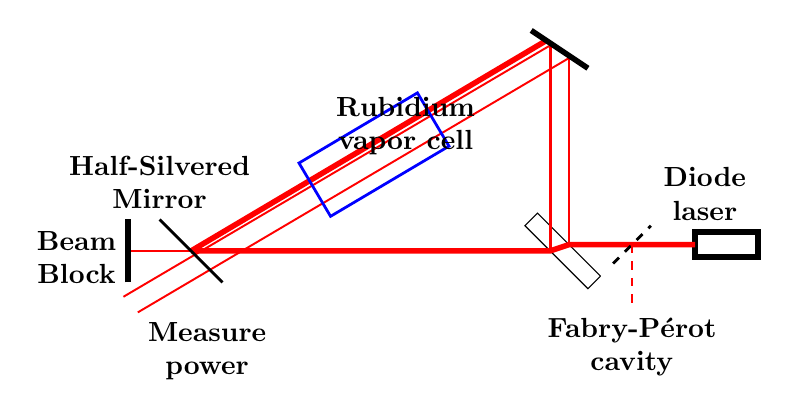
\begin{tikzpicture}[scale=.8]
    \draw[line width=2] (1, -.2) rectangle (2, .2) node[above left, align=center] {\textbf{Diode}\\\textbf{laser}};
    \draw (-.5, -0.5) -- ++(-1, 1) -- ++(-.2, -.2) -- ++(1, -1) -- ++(.2, .2);

    \draw[red, line width=2] (1, 0) -- (-1, 0) -- ++(-.3, -.1) -- (-7, -.1);
    \draw[red, line width=.7] (-7, -.1) -- (-8, -.1);
    \draw[red, line width=2] (-7, -.1) -- (-1.36, 3.24);
    \draw[red, line width=1] (-1, 0) -- (-1, 3);
    \draw[red, line width=1] (-1.3, -.1) -- (-1.3, 3.2);
    \draw[red, line width=.7] (-1.27, 3.18) -- (-6.94, -.16) -- (-8.074, -.828);
    \draw[red, line width=.7] (-.97, 2.98) -- (-6.7, -.4) -- (-7.846, -1.076) node[below right, black, align=center] {\textbf{Measure}\\\textbf{power}};

    \draw[line width=1, dashed] (-.3, -.3) -- (.3, .3);
    \draw[red, dashed, line width=1] (0, 0) -- (0, -1) node[black, below, align=center] {\textbf{Fabry-P\'erot}\\\textbf{cavity}};
    \draw[line width=2] (-.7, 2.8) -- (-1.6, 3.4);
    \draw[line width=2] (-8, -.6) --  (-8, .4) node[black, below left, align=center] {\textbf{Beam}\\\textbf{Block}};
    \draw[line width=1] (-6.5, -.6) --  (-7.5, .4) node[black, above, align=center] {\textbf{Half-Silvered}\\\textbf{Mirror}};

    \draw[blue, line width=1] (-2.906, 1.563) -- (-4.786, 0.449) -- (-5.287, 1.295) -- (-3.407, 2.409) -- cycle node[black, above left, align=center] {\textbf{Rubidium}\\\textbf{vapor cell}};
  \end{tikzpicture}
  \caption{A sketch of the experiment apparatus. (Some mirrors and other elements that are not important to the beam path as well as some measuring devices are not drawn in the plot for simplicity.)}
  \label{apparatus}
\end{figure}

Figure \ref{apparatus} shows the main beam path of this experiment. The $40mW$ diode laser is partially reflected by a half-silvered mirror into a rubidium vapor cell as the pump beam to pump atoms into the excited state. Two weak beams of the similar power are split from the main beam using a prism and are also sent to the cell. One of them, the probe beam, is overlap with the pump beam in order to satisfy the condition for saturated absorption spectroscopy and the other beam, the reference beam, is used to measure the absorption without the probe beam. The power of the two beams are measured separately. After balancing the power of the probe and the reference beams without the pump beam, the difference of the power between the probe and the reference beams can be used to measure the Lamb dips without the Doppler broadened baseline.

\subsection{Frequency scan and measurement.}
The frequency scan in this experiment is done by changing the current of the laser diode as well as moving the position and angle of the built-in feed back grading inside the diode laser. The temperature can also be used to change the frequency of the laser at a larger scale.

Since the goal of the experiment is measuring the energy level splitting, only relative frequency shift is important and need to be measured. This is done using a Fabry-P\'erot cavity on a weak beam taken from the main one using a beam splitter. The resonance condition of a Fabry-P\'erot cavity's lowest mode at which the transmission is maximized is,
\eqar{
  \nu=&\frac{c}{2nL}k
}
where $L$ the length of the cavity, $n$ the index of refraction, $c$ the speed of light, $k$ a arbitrary positive integer. The free spectral range of the cavity is defined as the separation between resonance peaks,
\eqar{
  f_{FSR}=&\frac{c}{2nL}
}
When scanning the frequency, the transmission of the cavity will be changing periodically. By comparing the frequency change with the free spectral range of the cavity, we can measure the frequency change in the scanning.
\begin{figure}
  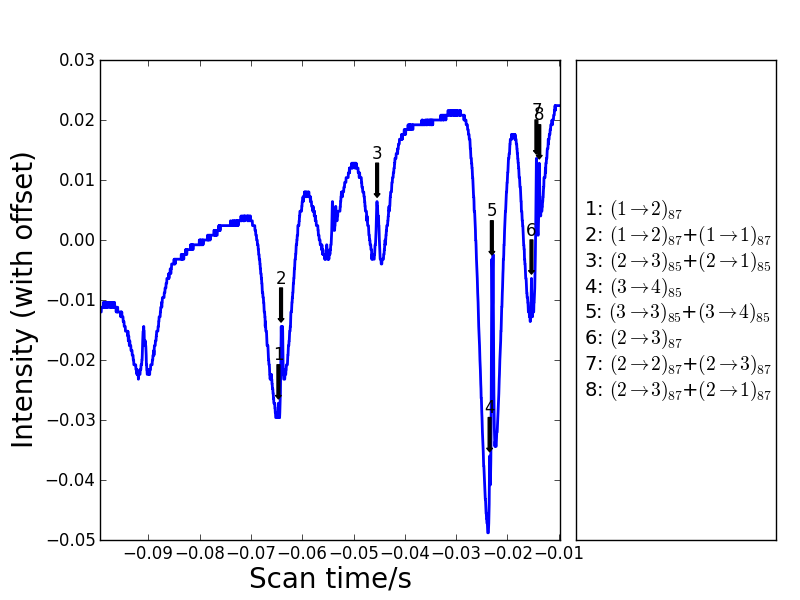
\includegraphics[width=8cm]{../all_data/4-18/20130418-14_12_48_probe.png}
  \caption{Probe beam intensity when scanning through the whole spectral range. The intensity is in arbitrary unit and is shifted to zero average. Dips are marked with the $F$ number of the ground state and the excited state. Crossover dips are marked with the two corresponding transitions.}
  \label{whole_probe}
\end{figure}

\begin{figure}
  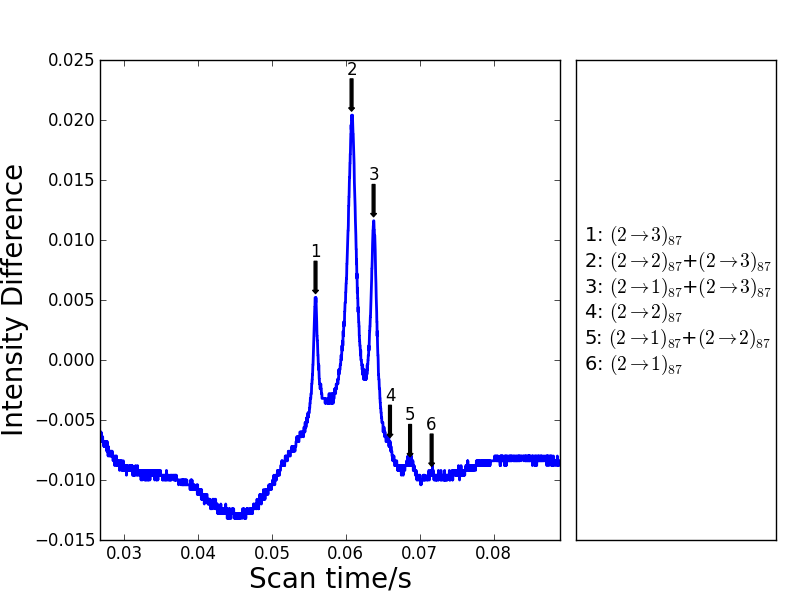
\includegraphics[width=8cm]{../all_data/4-18/20130418-12_52_13_balance.png}
  \caption{Difference between probe beam and reference beam intensity when scanning through the $F=2$ peak of rubidium $87$. Dips labelling is the same with figure \ref{whole_probe}}
  \label{rb87_diff}
\end{figure}

\begin{figure}
  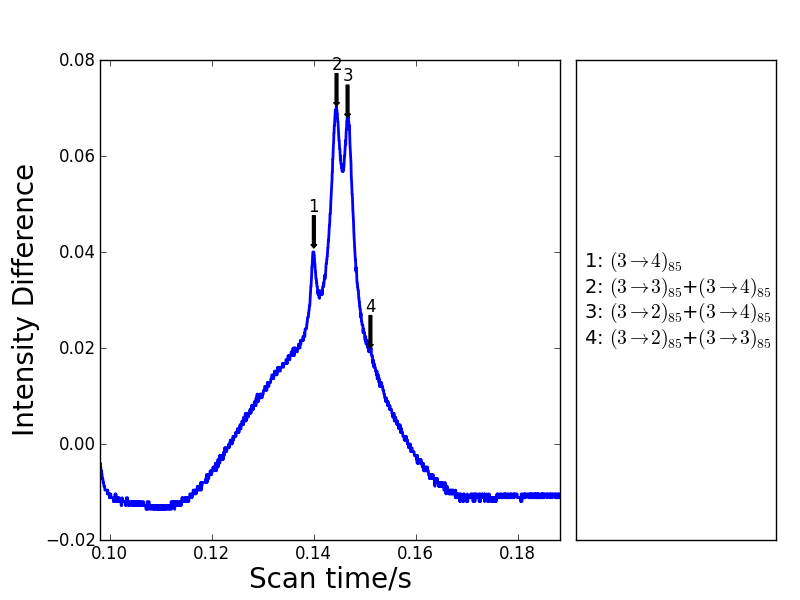
\includegraphics[width=8cm]{../all_data/4-18/20130418-13_0_10_balance_2.png}
  \caption{Difference between probe beam and reference beam intensity when scanning through the $F=3$ peak of rubidium $85$. Dips labelling is the same with figure \ref{whole_probe} and \ref{rb87_diff}.}
  \label{rb85_diff}
\end{figure}

\section{Measurement and hyperfine structure constant}
\subsection{Peaks identification}
Figure \ref{whole_probe} shows a scan of laser frequency over the whole range of interest. Six resolvable Doppler broadened absorption peaks can be seen in the signal. By comparing the separation of these peaks as well as the Lamb dips within each one and using the fact that the higher energy (therefore lower ground state energy and lower $F$) lines have a smaller excited state hyperfine splitting, we can identify the first, second, third and fifth peaks as the ${}^{87}Rb$ $F=2$, ${}^{85}Rb$ $F=3$, ${}^{85}Rb$ $F=2$ and ${}^{87}Rb$ $F=1$ transitions. The smaller fourth and sixth peaks in the measurement may be caused absorption of other materials or by side bands in the laser spectrum but we have not found a good way to test them.

Figure \ref{rb87_diff} shows the difference between the probe and reference signal during a scan of laser frequency over the right most absorption peak corresponding to the  ${}^{87}Rb$ $F=2$ transition. Four clear peaks and two barely visible peaks can be identified in the signal. The transition(s) each peaks correspond to is listed on the right of the plot. By deciding the position of each peaks, we can clearly see that the crossover peaks ($2$, $3$ and $5$) are right in the middle of the ``real'' peaks ($1$, $4$ and $6$) which corresponding to real transitions. It also proofs that the amplitude of the crossover peaks are a lot more larger and easier to measure than the ``real'' ones.

Figure \ref{rb85_diff} is another example of the difference signal between the probe and reference signal during a scan of laser frequency over the right most absorption peak corresponding to the  ${}^{85}Rb$ $F=3$ transition. Not all the peaks are visible in the signal and this is a good example of how we can identify and use the crossover peaks to determine the position of the ``real'' peaks because the largest two peaks in a measurement must be crossover peaks.

\subsection{Hyperfine structure constants.}

\begin{table}
  \begin{tabular}{|c|c|c|c|c|}
    \hline
    Isotope&Constant&Measured&Expected\cite{rubidium85_data,rubidium87_data}&Deviation\\\hline
    &$A_{5^2S_{1/2}}$&$0.986(40)GHz$&$1.0119GHz$&$0.6\sigma$\\\cline{2-5}
    ${}^{85}Rb$&$A_{5^2P_{3/2}}$&$24.44(81)MHz$&$25.0020(99)MHz$&$0.7\sigma$\\\cline{2-5}
    &$B_{5^2P_{3/2}}$&$32.2(4.8)MHz$&$25.790(93)MHz$&$1.3\sigma$\\\hline
    &$A_{5^2S_{1/2}}$&$3.285(65)GHz$&$3.4173GHz$&$2\sigma$\\\cline{2-5}
    ${}^{87}Rb$&$A_{5^2P_{3/2}}$&$84.58(52)MHz$&$84.7185(20)MHz$&$0.2\sigma$\\\cline{2-5}
    &$B_{5^2P_{3/2}}$&$16.03(80)MHz$&$12.4965(37)MHz$&$4\sigma$\\\hline
  \end{tabular}
  \caption{Measured values of the hyperfine structure constants of both excited and ground states comparing to expected values. Note: the expected values of the two $A_{5^2S_{1/2}}$ constants are not included because the measured uncertainties of them are so small that there is not enough space to include all significant digits.}
  \label{hfs_const}
\end{table}

After measuring the difference signal when zooming the scan in to each of the four Doppler broadened peaks shown in figure \ref{whole_probe} including figure \ref{rb85_diff} and \ref{rb87_diff}, we measured the splitting between the peaks using the periodic signals from the Fabry-P\'erot cavity (not shown on the plot) and calculated the hyperfine splitting constants of the excited states $A_{5^2P_{3/2}}$ and $B_{5^2P_{3/2}}$.

By doing the same on the visible peaks (mostly crossover peaks) in the whole region scan (figure \ref{whole_probe}) and using the result from the previous measurement of the excited state to correct for excited state shifting, we measured the hyperfine splitting of the ground states and calculated the ground hyperfine structure constants $A_{5^2S_{1/2}}$ of both isotopes.

The result of these measurement as well as the comparison to the expected values are shown in table \ref{hfs_const}. Most of the result are within a reasonable deviation $2\sigma$ from the expected value except $B_{5^2P_{3/2}}$ of ${}^{87}Rb$ which has a slightly larger $4\sigma$ standard deviation.

The error and uncertainty of the measurement mainly comes from deciding the positions of the peaks, the precision of the oscilloscope, which can only save data to files at a lower resolution and the temperature fluctuation of the laser diode, which will shift the frequency making it hard to do repeated measurement.

\section{Conclusion}
In this experiment, we finished our goal of doing Doppler-free spectrum measurement of rubidium $D_2$ transition. By measuring the frequency difference between different hyperfine splitting lines, we measured the hyperfine structure constants of all the related states and get a result within a reasonable deviation with the expected values.

\bibliography{report}
\end{document}
